\documentclass[11pt,aspectratio=169]{beamer}

% Assets
\usepackage[czech]{babel}				% Jazyk
\usepackage[a-2u]{pdfx}					% Kopírování z pdfka
\usepackage{tikz}						% Schémata automatů
\usepackage{csquotes}					% české uvozovky
\usepackage{enumerate}					% enumerate environment
\usepackage{indentfirst}
\usepackage{mathtools}
\usepackage{pifont}
\usepackage{xcolor}
\usepackage{enumitem,xcolor}
\usepackage{amsmath}
\usepackage[utf8]{inputenc}

\usepackage{listings}                   % Úryvky z kódu (C#)
\lstset{language=[Sharp]C, frame=lr}
% Enumerate
%\setlist[enumerate]{topsep=0pt,itemsep=-1ex,partopsep=1ex,parsep=1ex,label=(\arabic*)}

\MakeOuterQuote{"}

% Colors
\definecolor{lightblue}{HTML}{009AD4}
\definecolor{darkgreen}{HTML}{0D7103}
\definecolor{lightgreen}{HTML}{68FF00}
\definecolor{darkred}{HTML}{AF0B0B}
\definecolor{lightred}{HTML}{FF5100}
\definecolor{orange}{HTML}{FFE000}
\definecolor{codeblue}{HTML}{FF0055}
\definecolor{codegreen}{rgb}{0,0.6,0}
\definecolor{codegray}{rgb}{0.5,0.5,0.5}
\definecolor{codebeige}{HTML}{D4A000}
\definecolor{backcolour}{rgb}{0.95,0.95,0.92}

\newcommand{\markred}[1]{\textcolor{lightred}{#1}}
\newcommand{\markgreen}[1]{\textcolor{lightgreen}{#1}}
\newcommand{\markorange}[1]{\textcolor{orange}{#1}}
\newcommand{\markblue}[1]{\textcolor{lightblue}{#1}}

% Inline images
\newcommand{\inlineimgscale}{1.1}

% X and check mark
\newcommand{\cmark}{\markgreen{\ding{51}}}
\newcommand{\xmark}{\markred{\ding{55}}}

% Redefinions
\renewcommand{\implies}{\Rightarrow}
\renewcommand{\impliedby}{\Leftarrow}

% Math
\newcommand{\R}{\mathbb{R}}
\newcommand{\C}{\mathbb{C}}
\newcommand{\N}{\mathbb{N}}
\newcommand{\Z}{\mathbb{Z}}
\newcommand{\Q}{\mathbb{Q}}

% Code
\lstdefinestyle{clang}{
    basicstyle=\small\ttfamily\color{white},
    language=C,
    keywordstyle=\color{codeblue},
    commentstyle=\color{codegreen},
    numberstyle=\tiny\color{codegray},
    stringstyle=\color{codebeige},
    breakatwhitespace=false,
    breaklines=true,
    captionpos=b,
    keepspaces=true,
    numbersep=5pt,
    showspaces=false,
    showstringspaces=false,
    showtabs=false,
    morekeywords={void,int,double,float,unsigned,if,else,\#include}
    tabsize=0.5
}
\lstset{escapeinside={(*}{*)},style=clang}

\newcommand{\hlcode}[1]{\colorbox{red}{#1}}
% Beamer theme
\usetheme{Boadilla}
\setbeamertemplate{frame numbering}[fraction]
\usecolortheme[named=black]{structure}
\setbeamertemplate{navigation symbols}{}
\setbeamerfont{title}{series=\bfseries,parent=structure}
\setbeamerfont{frametitle}{series=\bfseries,parent=structure}
\usefonttheme[onlymath]{serif}
\urlstyle{same}

% Dark theme
\setbeamercolor{frametitle}{fg=white}
\setbeamercolor{title}{fg=white}
\setbeamercolor{background canvas}{bg=black}
\setbeamercolor{normal text}{fg=white}

\defbeamertemplate*{title page}{customized}[1][]
{ 
  \usebeamerfont*{title}\inserttitle\par
  \bigskip
  \usebeamerfont*{subtitle}\textit{\insertsubtitle}\par
  \bigskip \bigskip \bigskip \bigskip 
  \usebeamerfont{author}\insertauthor\par
  \usebeamerfont{institute}Kabinet \office\\\url{weber3@spsejecna.cz}\bigskip
}

% Title page
\title{Práce s plošnými strukturogramy}
\def\spacing{0.7em}
\def\bigspacing{5em}

\begin{titlepage}
    \begin{center}
        \vspace*{\fill}
        \Huge{\textbf{\maintitle}}\\
        \huge{\subtitle}\\
        \vspace*{\spacing}
        \large{\textbf{\authorname}}\\
        \vspace*{\spacing}
        \large{\textsc{\institution}}\\
        \vspace*{\bigspacing}
        \vspace*{\fill}
        \large{\textit{Poslední aktualizace:} \currentdate}
    \end{center}
    \pagenumbering{arabic}
    \normalsize
\end{titlepage}

\begin{document}

    \section{Opakování}
    \begin{frame}[t]
        \titlepage
    \end{frame}

    \begin{frame}[t]{Nejdříve zopáčko...}
        \only<2->{Co vypíše program níže?}
        \only<3->{\begin{figure}
            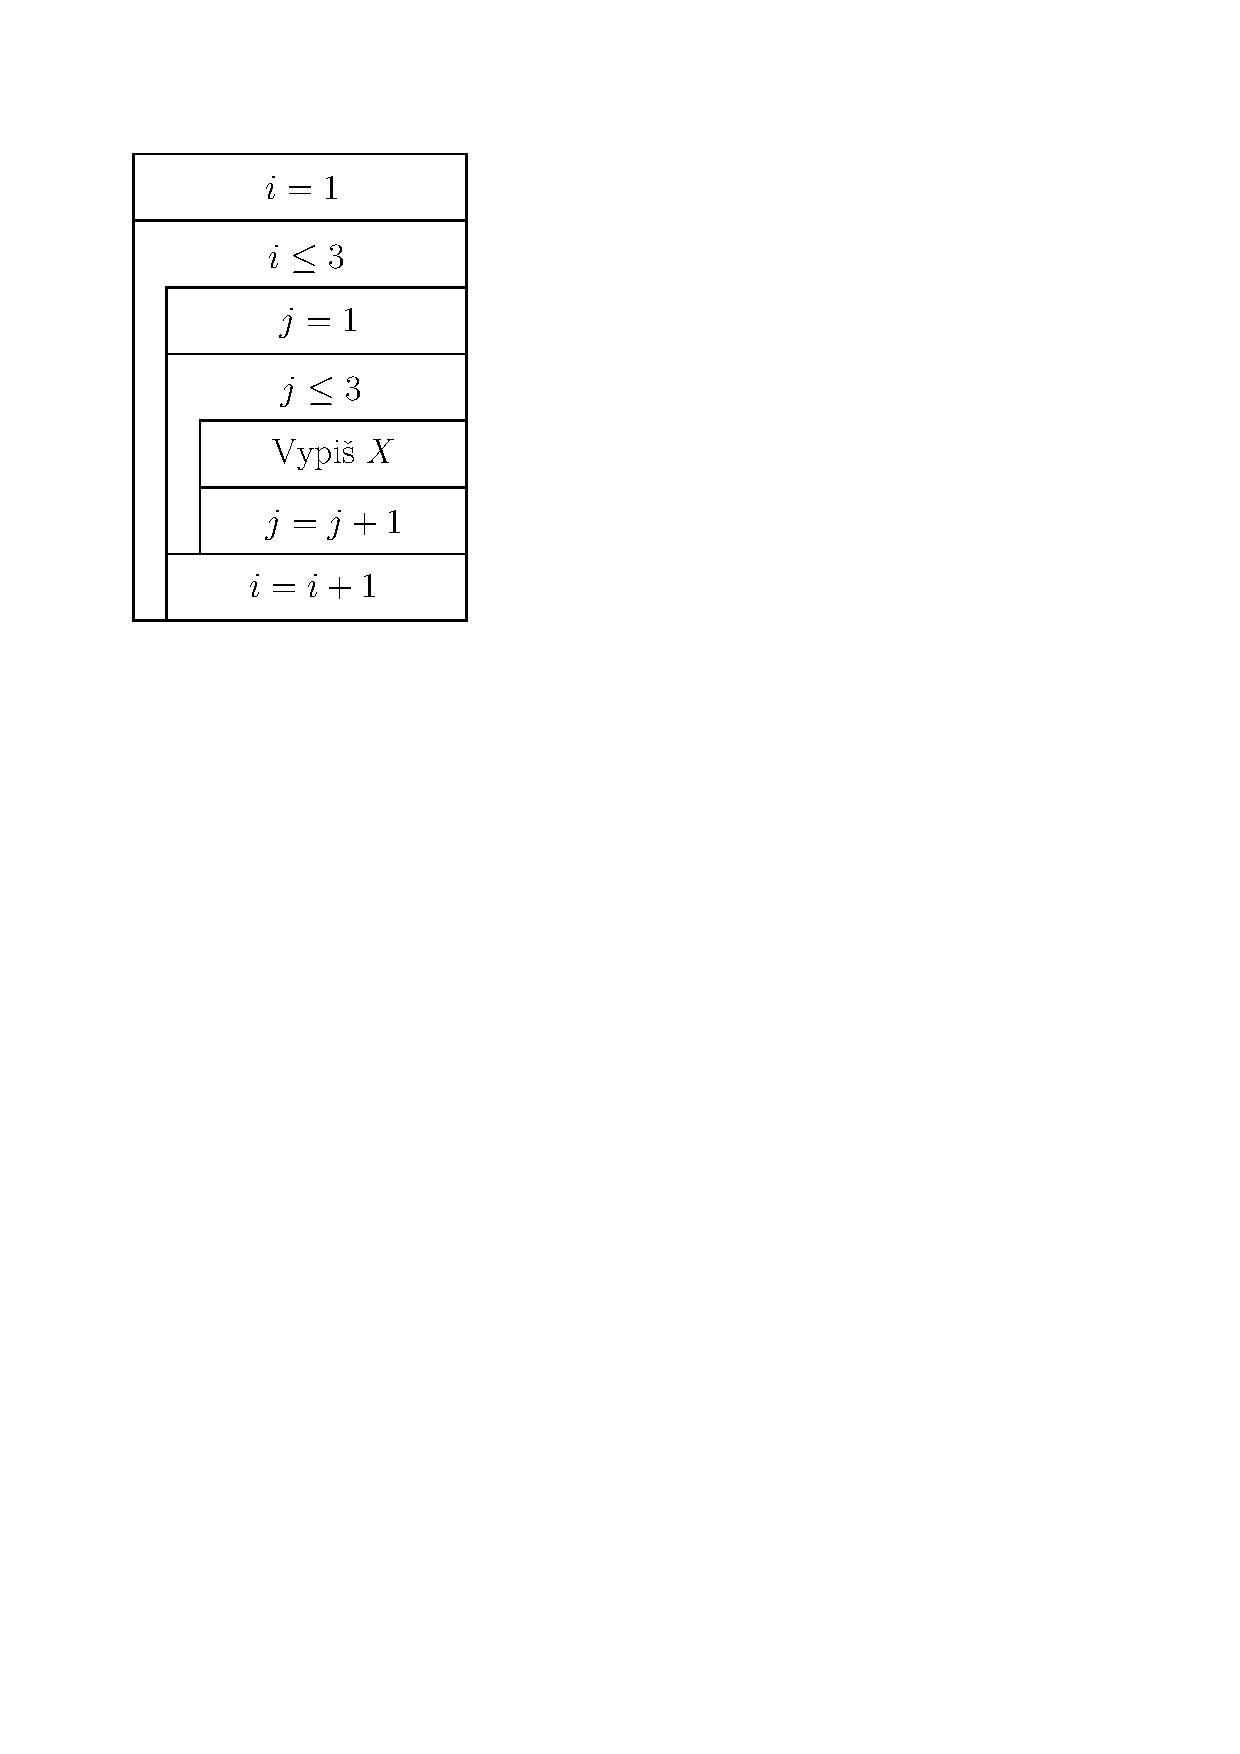
\includegraphics[scale=.7]{../images/01-priklad1_opakovani.pdf}
        \end{figure}}
    \end{frame}

    \begin{frame}[t]{Nejdříve zopáčko...}
        \only<2->{Výstup bude XXXXXXXXX.}
        \only<3->{\begin{center}
            \[\underbrace{\overbrace{\markgreen{XXX}}^{i=1}\;\overbrace{\markred{XXX}}^{i=2}\;\overbrace{\markorange{XXX}}^{i=3}}_{\text{9-krát}}.\]
        \end{center}}
        \only<4->{Pro každé opakování vnější iterace se vnitřní iterace provede třikrát $\implies$ $3\cdot 3=9$.}
    \end{frame}

    \section{Příklad s výstupem}
    \begin{frame}[t]{Upravená varianta}
        \only<2->{Zkusme program trochu upravit. Jak se změní výstup programu, bude-li vnitřní iterace \textbf{s testem na konci}?}
        \only<3->{\begin{figure}
            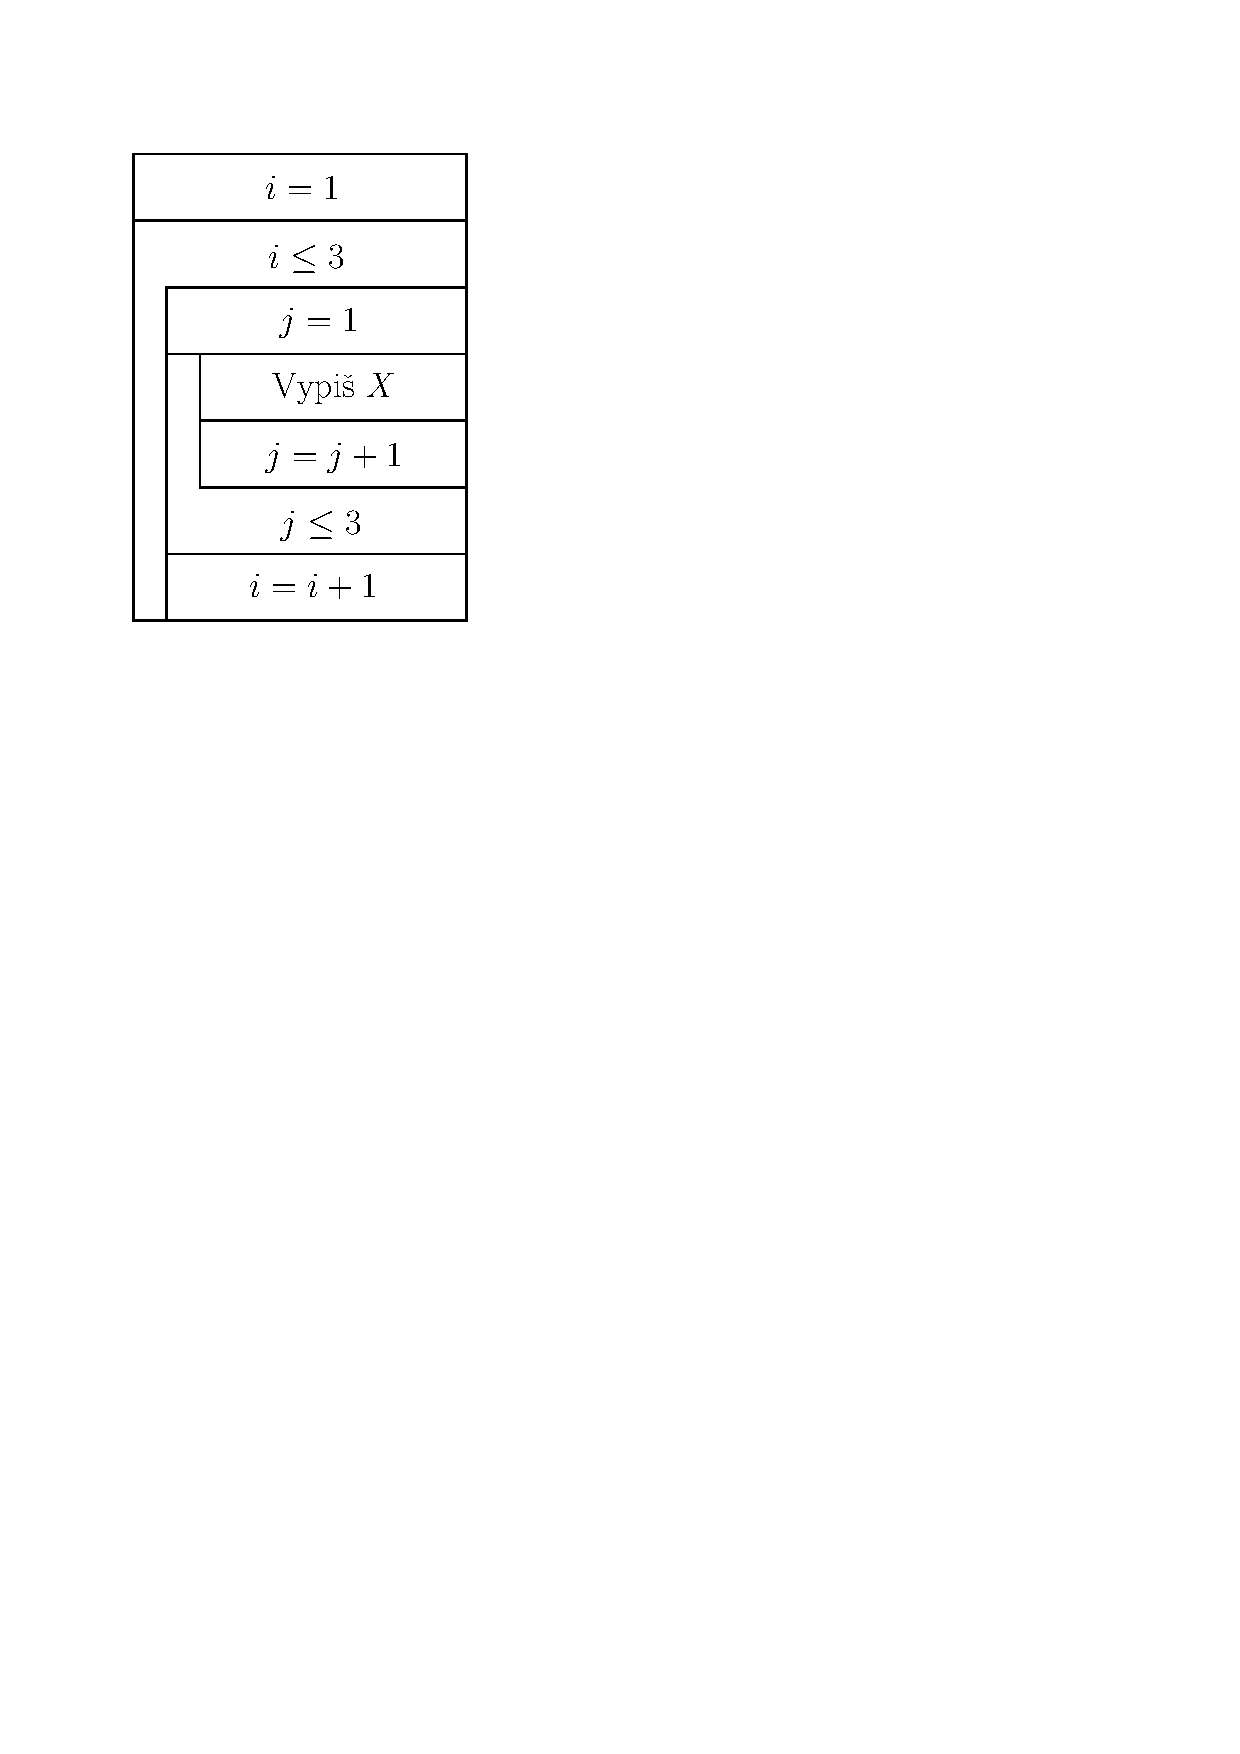
\includegraphics[scale=.7]{../images/01-priklad2_opakovani.pdf}
        \end{figure}}
    \end{frame}

    \begin{frame}{Upravená varianta}
        Kód vnitřní iterace se provede opět třikrát $\implies$ \markgreen{výstup bude stejný. \emoji{slightly-smiling-face}}
    \end{frame}

    \section{Obecný vstup}
    \begin{frame}[t]{Obecný vstup}
        \only<2->{Zkusme program zobecnit. Nechceme, aby počet vypsaných symbolů byl vždy pevný\dots}
        \only<3->{\begin{center}
            $\implies$ \markgreen{PŘIDÁME UŽIVATELSKÝ VSTUP}
        \end{center}}
        \only<4->{Program se na začátku zeptá uživatele na jisté číslo $n$, s nímž pak dále pracuje.}
    \end{frame}

    \begin{frame}{Obecný vstup}
        \begin{figure}
            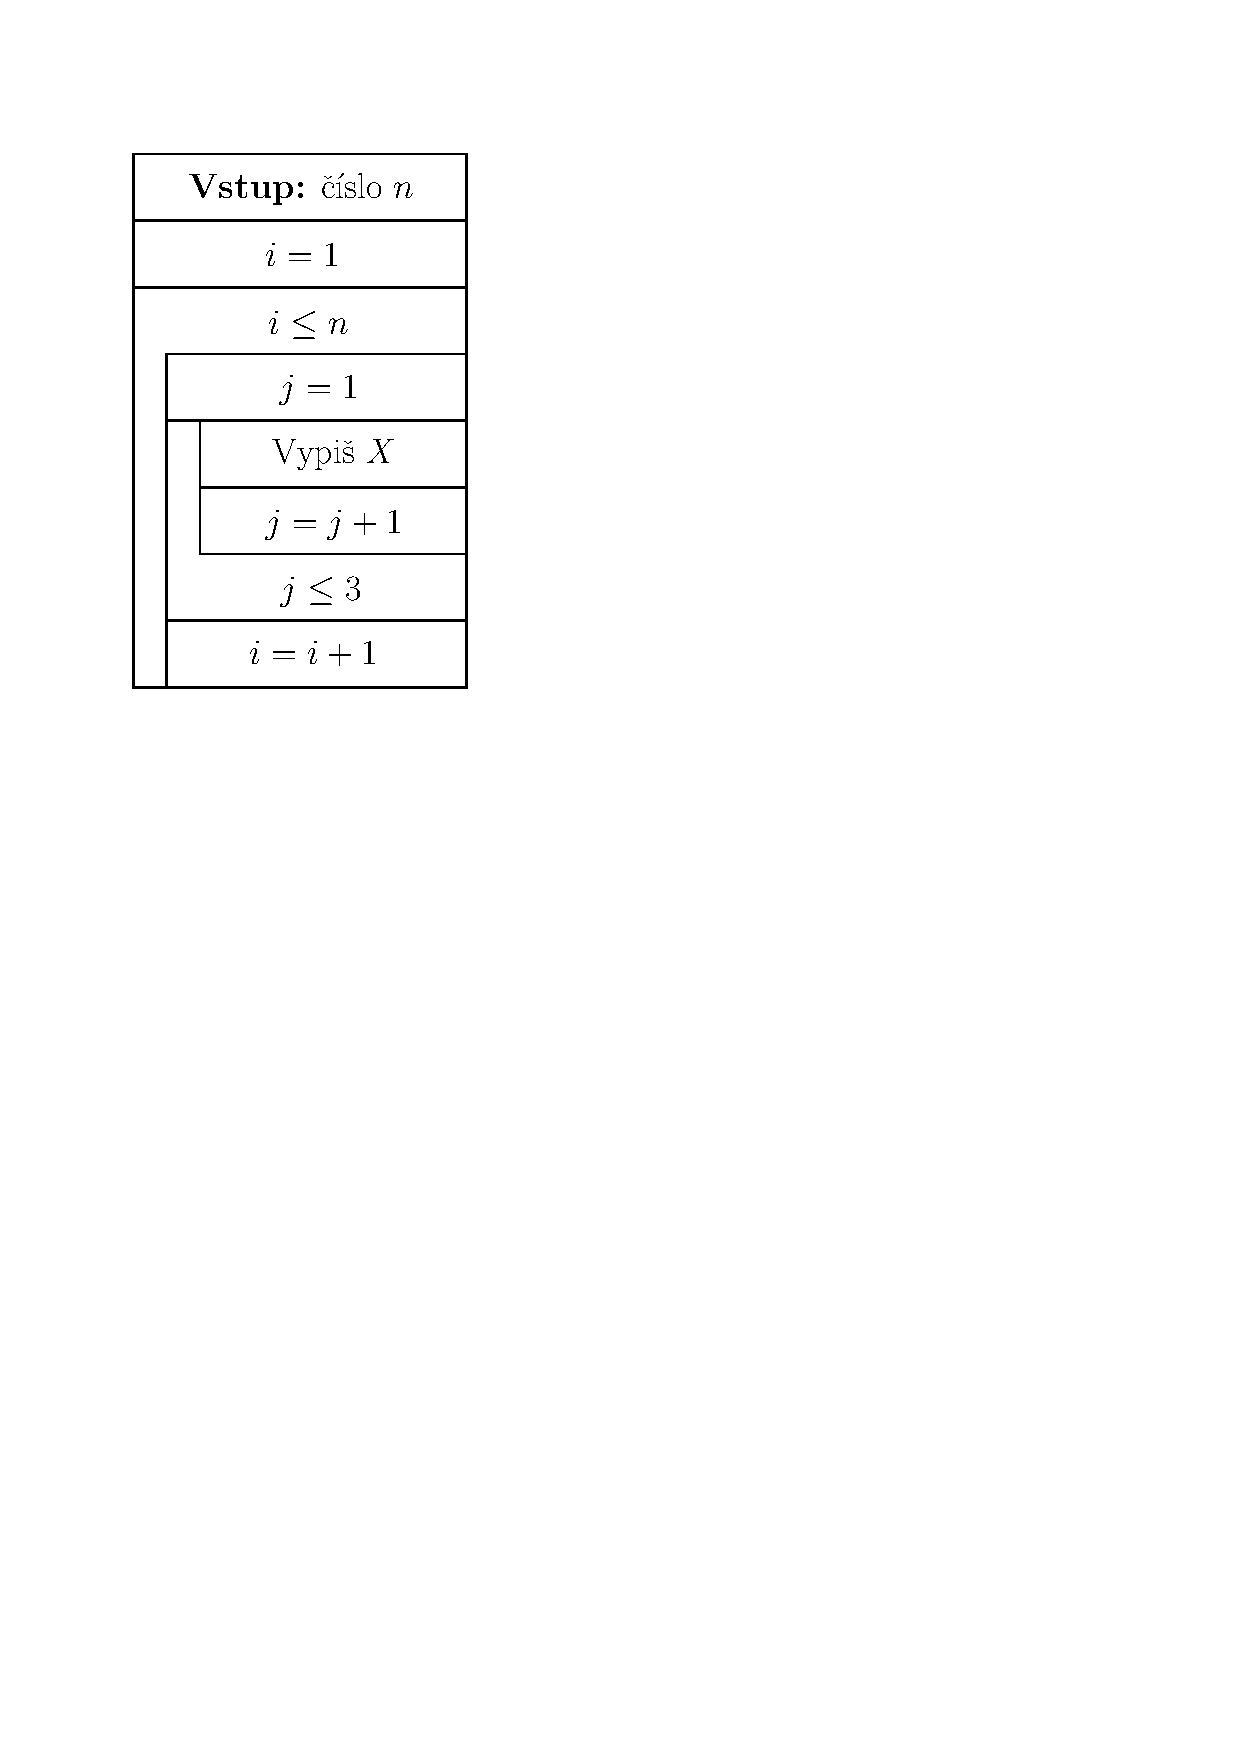
\includegraphics[scale=.7]{../images/01-priklad3_opakovani.pdf}
        \end{figure}
    \end{frame}

    \begin{frame}[t]
        \only<2->{Počet vypsaných symbolů \textit{X} již není pevný (je závislý na hodnotě $n$).\\}
        \only<3->{Vnější iterace se nyní provede $n$-krát a pro každé její opakování se vnitřní iterace provede právě třikrát.}
        \only<4->{\begin{center}
            \[\underbrace{\overbrace{\markgreen{XXX}}^{i=1}\;\overbrace{\markred{XXX}}^{i=2}\;\overbrace{\markorange{XXX}}^{i=3}\;\overbrace{\markgreen{XXX}}^{i=4}\;\cdots\;\overbrace{\markorange{XXX}}^{i=n}}_{\text{??}}\]
        \end{center}}
        \only<5->{$\implies$ $n\cdot 3=\markgreen{3n}$ symbolů X.}
    \end{frame}

    \section{Samostatná práce}
    \begin{frame}[t]{Samostatná práce}
        \only<2->{Kolik symbolů X vypíše tento program?}
        \only<3->{\begin{figure}
            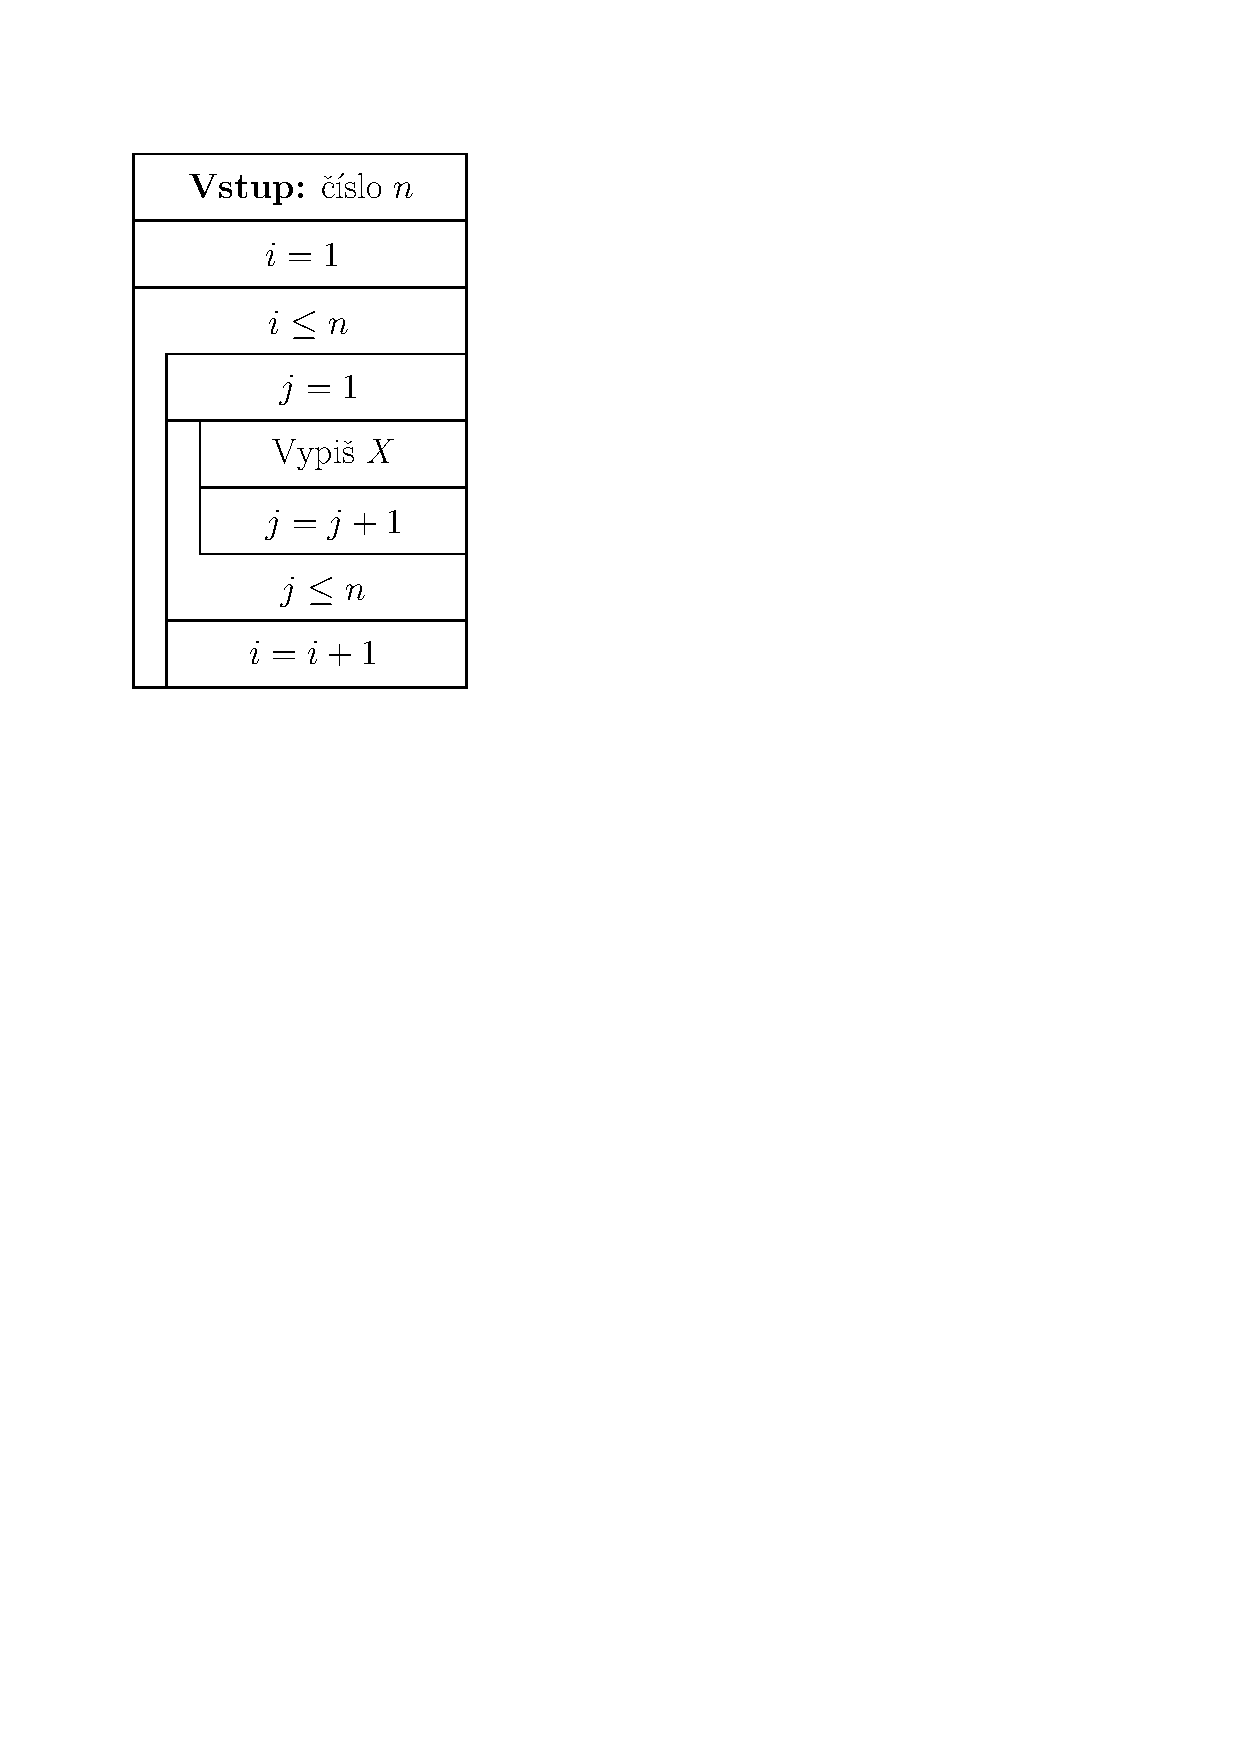
\includegraphics[scale=.7]{../images/01-priklad4_opakovani.pdf}
        \end{figure}}
    \end{frame}

    \begin{frame}
        \only<2->{\begin{center}
            \[\overbrace{\markgreen{XXX\dots X}}^{n}\;\overbrace{\markred{XXX\dots X}}^{n}\;\overbrace{\markorange{XXX\dots X}}^{n}\;\cdots\;\overbrace{\markgreen{XXX\dots X}}^{n}\]
        \end{center}}
        \only<3->{Pro každé opakování vnější iterace se vnitřní iterace se zopakuje $n$-krát} \only<3->{$\implies$ správná odpověď je $\markgreen{n\cdot n=n^2}$ symbolů X. \emoji{slightly-smiling-face}}
    \end{frame}

    \section{Závěr}
    \begin{frame}{Dotazy?}
        \begin{figure}
            \centering
            
\includegraphics[scale=.5]{../images/discussion.pdf}
        \end{figure}
    \end{frame}

\end{document}